\subsubsection{L'utilisation de la bibliothèque/framework Qt}
\begin{figure}[h]
\centering

\includegraphics{figures/Qt.png}
\caption{Logo du framework Qt, par Nokia.}
\label{Logo de Qt}
\end{figure}
Pour l'interface graphique de l'application, nous avons choisi d'utiliser le framework Qt de Nokia, qui propose un ensemble de bibliothèques permettant la conception d'interfaces graphiques en C++ de façon rapide et simple.

Nous avons également choisi d'utiliser Qt pour son coté multi plateforme: Ainsi, la bibliothèque est utilisable sur diverses plateformes: Windows, GNU/Linux, Mac OS, mais aussi Android ou Symbian pour le développement mobile, nous permettant de faire une version fonctionelle sur téléphone mobile, bien que non peaufinée. Par ailleurs, la bibliothèque s'intègre parfaitement dans tout les environnements de bureau (Notamment entre les bureaux Gnome 2/GTK sous Linux, KDE4 sous Linux, Gnome 3), en respectant les HIG (Human Interfaces Guidelines, règles de conception pour les interfaces graphiques ) de chaque interface.

Par ailleurs, pour nos besoins, l'utilisation du framework Qt était la plus appropriée, dans le sens où l'interface graphique a été relativement simple à concevoir, nous laissant plus de temps pour la partie algorithmique du programme.

\begin{figure}[p]
\centering
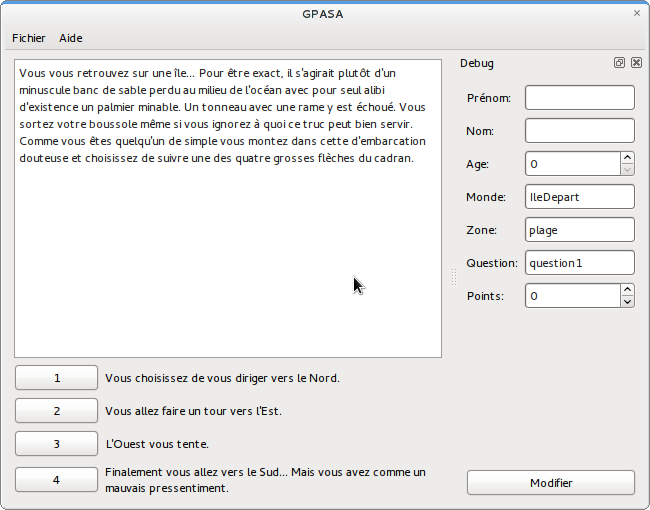
\includegraphics[scale=0.4]{figures/screenshots/gnome3}
\caption{Capture d'ecran de l'application tournant sous un systeme Linux sous Gnome 3.}
\label{CaptureGnome3}
\end{figure}

\begin{figure}[p]
\centering
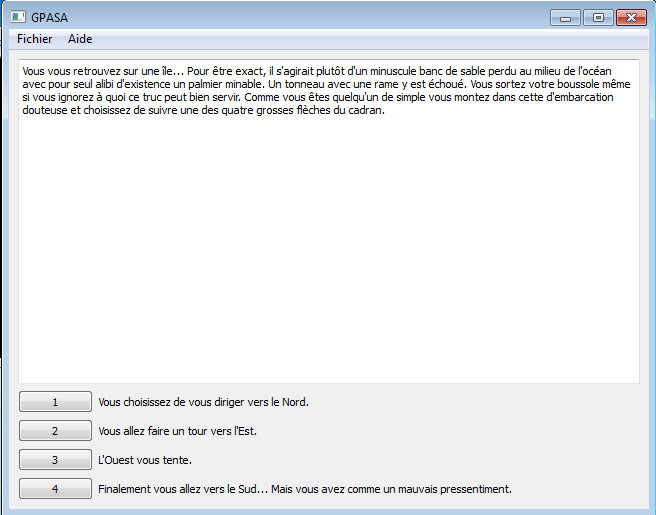
\includegraphics[scale=0.65]{figures/screenshots/windows7}
\caption{Capture d'ecran de l'application tournant sous un systeme Windows 7.}
\label{CaptureWindows7}
\end{figure}



\begin{figure}[p]
\centering
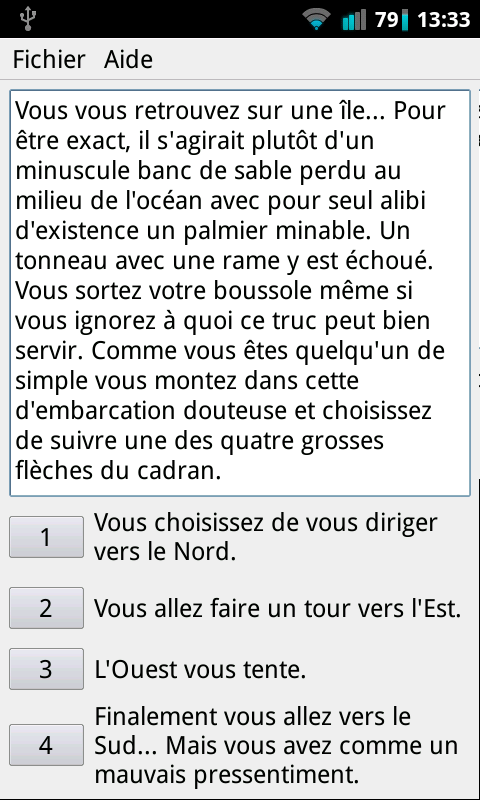
\includegraphics[scale=0.3]{figures/screenshots/androidWVGA}
\caption{Capture d'ecran de l'application tournant sur un téléphone sous Android 2.3.4}
\label{CaptureAndroid}
\end{figure}




\begin{figure}[p]
\centering
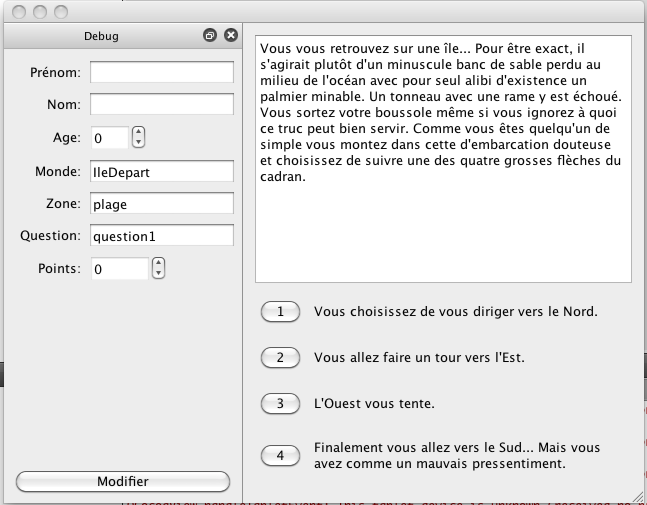
\includegraphics[scale=0.55]{figures/screenshots/OSX}
\caption{Capture d'ecran de l'application tournant sur Mac OS X}
\label{CaptureMac}
\end{figure}

\pagebreak